\chapter{Diagrama de conex\~oes el\'etricas da BeagleBone Black}
\label{Anexo1}

%Adiciona o PDF do diagrama esquemático da BBB
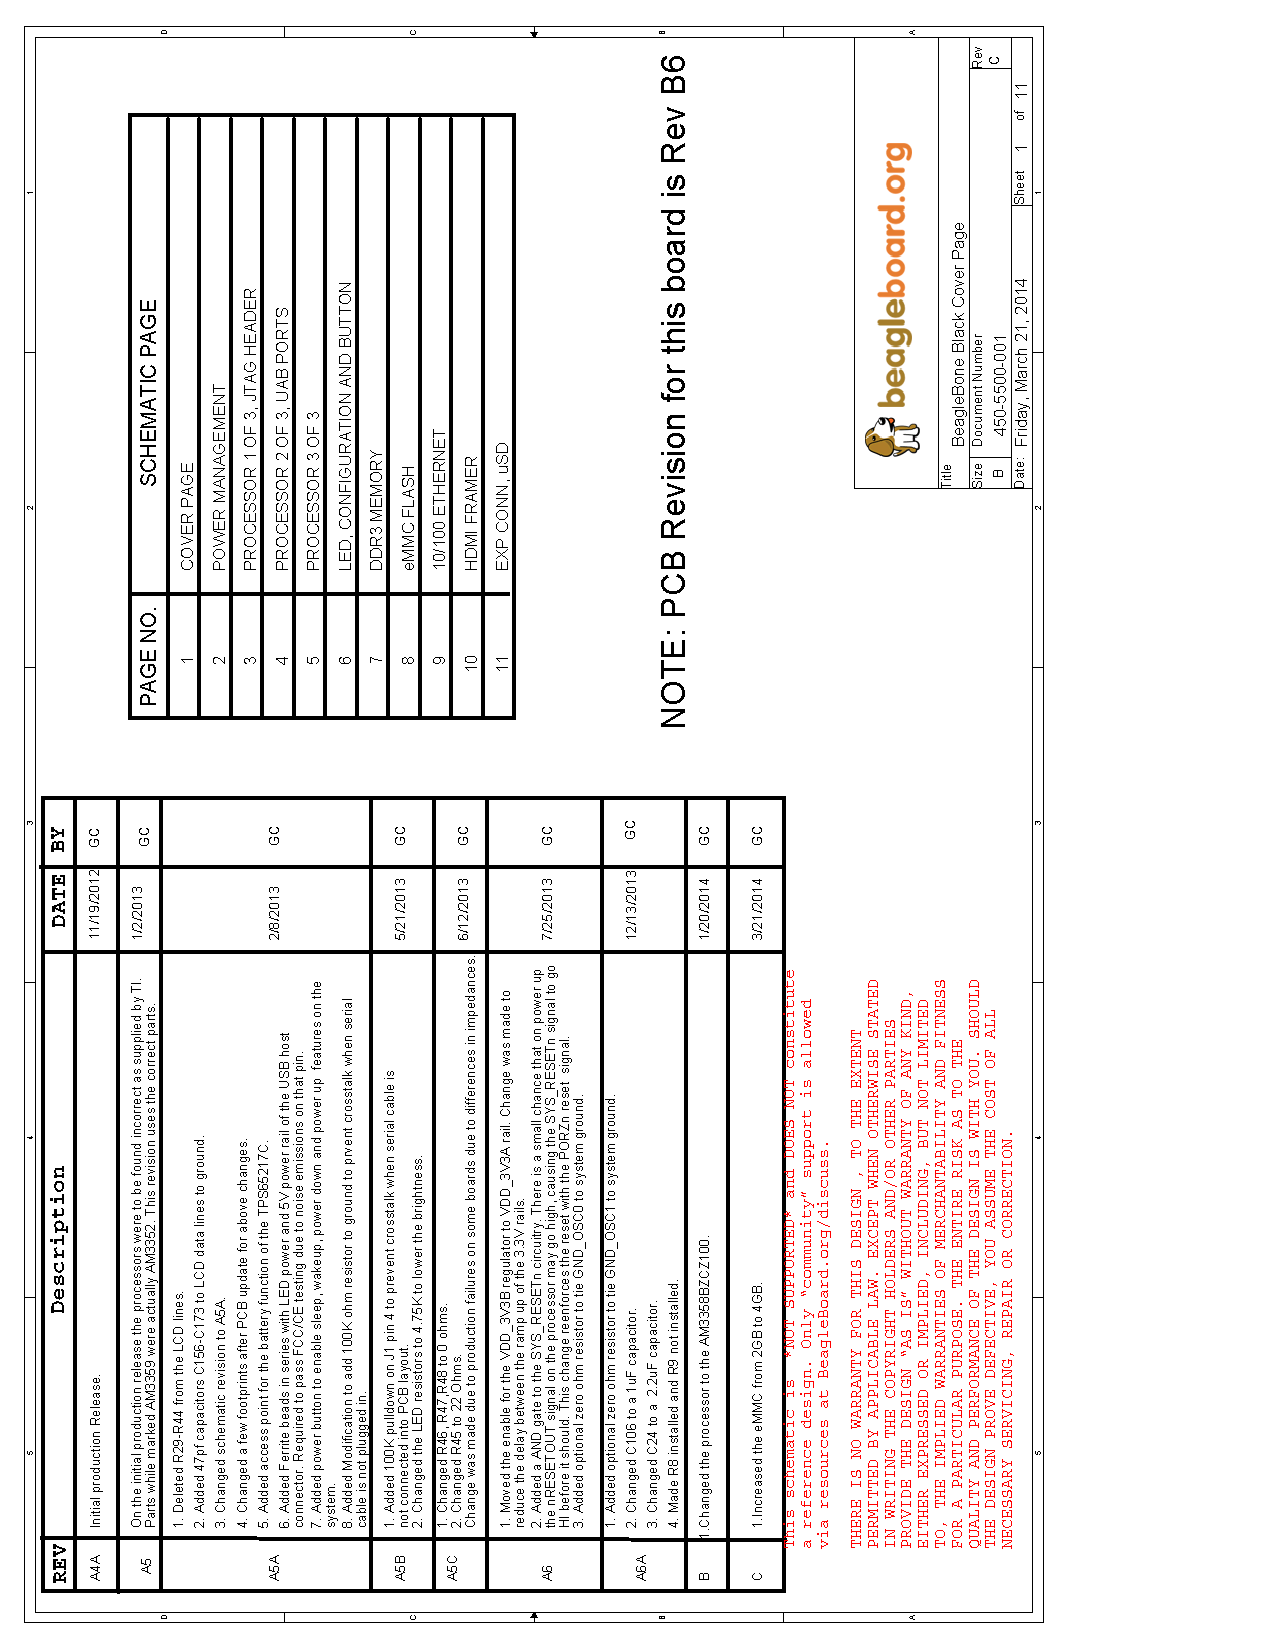
\includepdf[pages=-]{./Resources/BBB_SCH.pdf}

% % % % % % % % % % % % % % % % % % % % % % % % % % % % % % % % % % % % % % % % % % % % % % % % % % %
\chapter{Registradores do M\'odulo de Controle}
\label{Anexo2}


\begin{longtable}{ | M{7.5cm} | M{7.5cm} |}
	\captionsetup{justification=centering}
	\caption[Registradores do m\'odulo de controle]{Registradores do m\'odulo  de controle. \\Fonte: adaptado de TEXAS INSTRUMENTS(2014)}
	\label{dt_offset}\\
	\endfirsthead
		\caption[]{Registradores do m\'odulo  de controle. \\Fonte: adaptado de TEXAS INSTRUMENTS(2014) (continua\c{c}\~ao)}
	\endhead
	\hline
	\textbf{Offset} & \textbf{Acr\^onimo} \\ \hline
	800h & conf\_gpmc\_ad0 \\ \hline
	804h & conf\_gpmc\_ad1 \\ \hline
	808h & conf\_gpmc\_ad2 \\ \hline
	80Ch & conf\_gpmc\_ad3 \\ \hline
	810h & conf\_gpmc\_ad4 \\ \hline
	814h & conf\_gpmc\_ad5 \\ \hline
	818h & conf\_gpmc\_ad6 \\ \hline
	81Ch & conf\_gpmc\_ad7 \\ \hline
	820h & conf\_gpmc\_ad8 \\ \hline
	824h & conf\_gpmc\_ad9 \\ \hline
	828h & conf\_gpmc\_ad10 \\ \hline
	82Ch & conf\_gpmc\_ad11 \\ \hline
	830h & conf\_gpmc\_ad12 \\ \hline
	834h & conf\_gpmc\_ad13 \\ \hline
	838h & conf\_gpmc\_ad14 \\ \hline
	83Ch & conf\_gpmc\_ad15 \\ \hline
	840h & conf\_gpmc\_a0 \\ \hline
	844h & conf\_gpmc\_a1 \\ \hline
	848h & conf\_gpmc\_a2 \\ \hline
	84Ch & conf\_gpmc\_a3 \\ \hline
	850h & conf\_gpmc\_a4 \\ \hline
	854h & conf\_gpmc\_a5 \\ \hline
	858h & conf\_gpmc\_a6 \\ \hline
	85Ch & conf\_gpmc\_a7 \\ \hline
	860h & conf\_gpmc\_a8 \\ \hline
	864h & conf\_gpmc\_a9 \\ \hline
	868h & conf\_gpmc\_a10 \\ \hline
	86Ch & conf\_gpmc\_a11 \\ \hline
	870h & conf\_gpmc\_wait0 \\ \hline
	874h & conf\_gpmc\_wpn \\ \hline
	878h & conf\_gpmc\_ben1 \\ \hline
	87Ch & conf\_gpmc\_csn0 \\ \hline
	880h & conf\_gpmc\_csn1 \\ \hline
	884h & conf\_gpmc\_csn2 \\ \hline
	888h & conf\_gpmc\_csn3 \\ \hline
	88Ch & conf\_gpmc\_clk \\ \hline
	890h & conf\_gpmc\_advn\_ale \\ \hline
	894h & conf\_gpmc\_oen\_ren \\ \hline
	898h & conf\_gpmc\_wen \\ \hline
	89Ch & conf\_gpmc\_ben0\_cle \\ \hline
	8A0h & conf\_lcd\_data0 \\ \hline
	8A4h & conf\_lcd\_data1 \\ \hline
	8A8h & conf\_lcd\_data2 \\ \hline
	8ACh & conf\_lcd\_data3 \\ \hline
	8B0h & conf\_lcd\_data4 \\ \hline
	8B4h & conf\_lcd\_data5 \\ \hline
	8B8h & conf\_lcd\_data6 \\ \hline
	8BCh & conf\_lcd\_data7 \\ \hline
	8C0h & conf\_lcd\_data8 \\ \hline
	8C4h & conf\_lcd\_data9 \\ \hline
	8C8h & conf\_lcd\_data10 \\ \hline
	8CCh & conf\_lcd\_data11 \\ \hline
	8D0h & conf\_lcd\_data12 \\ \hline
	8D4h & conf\_lcd\_data13 \\ \hline
	8D8h & conf\_lcd\_data14 \\ \hline
	8DCh & conf\_lcd\_data15 \\ \hline
	8E0h & conf\_lcd\_vsync \\ \hline
	8E4h & conf\_lcd\_hsync \\ \hline
	8E8h & conf\_lcd\_pclk \\ \hline
	8ECh & conf\_lcd\_ac\_bias\_en \\ \hline
	8F0h & conf\_mmc0\_dat3 \\ \hline
	8F4h & conf\_mmc0\_dat2 \\ \hline
	8F8h & conf\_mmc0\_dat1 \\ \hline
	8FCh & conf\_mmc0\_dat0 \\ \hline
	900h & conf\_mmc0\_clk \\ \hline
	904h & conf\_mmc0\_cmd \\ \hline
	908h & conf\_mmi1\_col \\ \hline
	90Ch & conf\_mmi1\_crs \\ \hline
	910h & conf\_mmi1\_rx\_er \\ \hline
	914h & conf\_mmi1\_tx\_en \\ \hline
	918h & conf\_mmi1\_rx\_dv \\ \hline
	91Ch & conf\_mmi1\_txd3 \\ \hline
	920h & conf\_mmi1\_txd2 \\ \hline
	924h & conf\_mmi1\_txd1 \\ \hline
	928h & conf\_mmi1\_txd0 \\ \hline
	92Ch & conf\_mmi1\_tx\_clk \\ \hline
	930h & conf\_mmi1\_rx\_clk \\ \hline
	934h & conf\_mmi1\_rxd3 \\ \hline
	938h & conf\_mmi1\_rxd2 \\ \hline
	93Ch & conf\_mmi1\_rxd1 \\ \hline
	940h & conf\_mmi1\_rxd0 \\ \hline
	944h & conf\_rmmi1\_ref\_clk \\ \hline
	948h & conf\_mdio \\ \hline
	94Ch & conf\_mdc \\ \hline
	950h & conf\_spi0\_sclk \\ \hline
	954h & conf\_spi0\_d0 \\ \hline
	958h & conf\_spi0\_d1 \\ \hline
	95Ch & conf\_spi0\_cs0 \\ \hline
	960h & conf\_spi0\_cs1 \\ \hline
	964h & conf\_ecap0\_in\_pwm0\_out \\ \hline
	968h & conf\_uart0\_ctsn \\ \hline
	96Ch & conf\_uart0\_rtsn \\ \hline
	970h & conf\_uart0\_rdx \\ \hline
	974h & conf\_uart0\_tdx \\ \hline
	978h & conf\_uart1\_ctsn \\ \hline
	97Ch & conf\_uart1\_rtsn \\ \hline
	980h & conf\_uart1\_rdx \\ \hline
	984h & conf\_uart1\_tdx \\ \hline
	988h & conf\_i2c0\_sda \\ \hline
	98Ch & conf\_i2c0\_scl \\ \hline
	990h & conf\_mcasp0\_aclkx \\ \hline
	994h & conf\_mcasp0\_fsx \\ \hline
	998h & conf\_mcasp0\_axr0 \\ \hline
	99Ch & conf\_mcasp0\_ahclkr \\ \hline
	9A0h & conf\_mcasp0\_aclkr \\ \hline
	9A4h & conf\_mcasp0\_fsr \\ \hline
	9A8h & conf\_mcasp0\_axr1 \\ \hline
	9ACh & conf\_mcasp0\_ahclkx \\ \hline
	9B0h & conf\_xdma\_event\_intr0 \\ \hline
	9B4h & conf\_xdma\_event\_intr1 \\ \hline
	9B8h & conf\_warmrstn \\ \hline
	9C0h & conf\_nnmi \\ \hline
	9D0h & conf\_tms \\ \hline
	9D4h & conf\_tdi \\ \hline
	9D8h & conf\_tdo \\ \hline
	9DCh & conf\_tck \\ \hline
	9E0h & conf\_trstn \\ \hline
	9E4h & conf\_emu0 \\ \hline
	9E8h & conf\_emu1 \\ \hline
	9F8h & conf\_rtc\_pwronrstn \\ \hline
	9FCh & conf\_pmic\_power\_en \\ \hline
	A00h & conf\_ext\_wakeup \\ \hline
	A04h & conf\_rtc\_kaldo\_enn \\ \hline
	A1Ch & conf\_usb0\_drvvbus \\ \hline
	A34h & conf\_usb1\_drvvbus \\ \hline
\end{longtable}

%%%%%%%%%%%%%%%%%%%%%%%%%%%%%%%%%%%%%%%%%%%%%%%%%%%%%%%%%%%%%%%%%%%%%%%%%%%%%

\chapter{V\'alvula Danfoss EV210BD 032U3620}
\label{Anexo3}

%Adiciona o PDF do diagrama esquemático da BBB
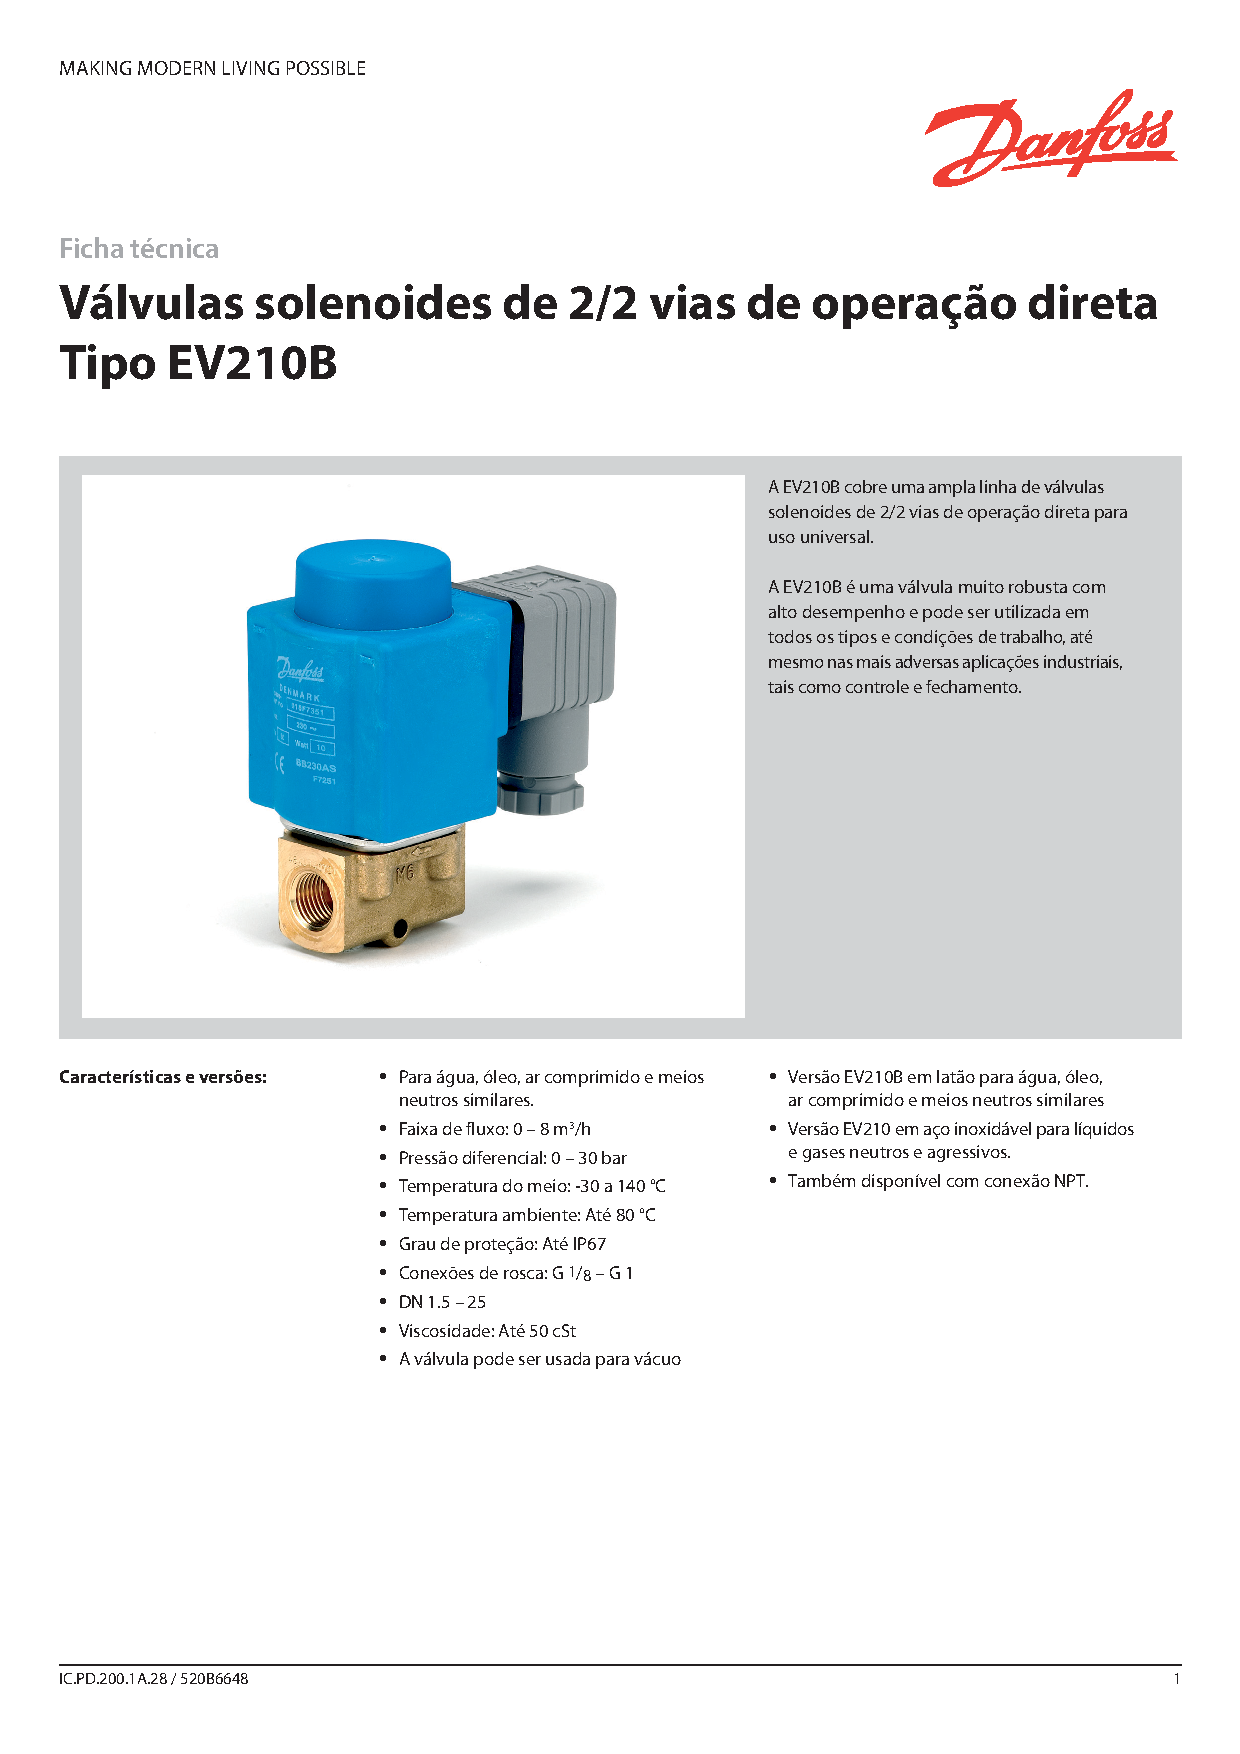
\includepdf[pages=1-2]{./Resources/valvula_datasheet.pdf}
\includepdf[pages={11,18,19,34}]{./Resources/ev210b.pdf}

%%%%%%%%%%%%%%%%%%%%%%%%%%%%%%%%%%%%%%%%%%%%%%%%%%%%%%%%%%%%%%%%%%%%%%%%%%%%%

\chapter{Bobina Danfoss 042N7550}
\label{Anexo4}

%Adiciona o PDF do diagrama esquemático da BBB
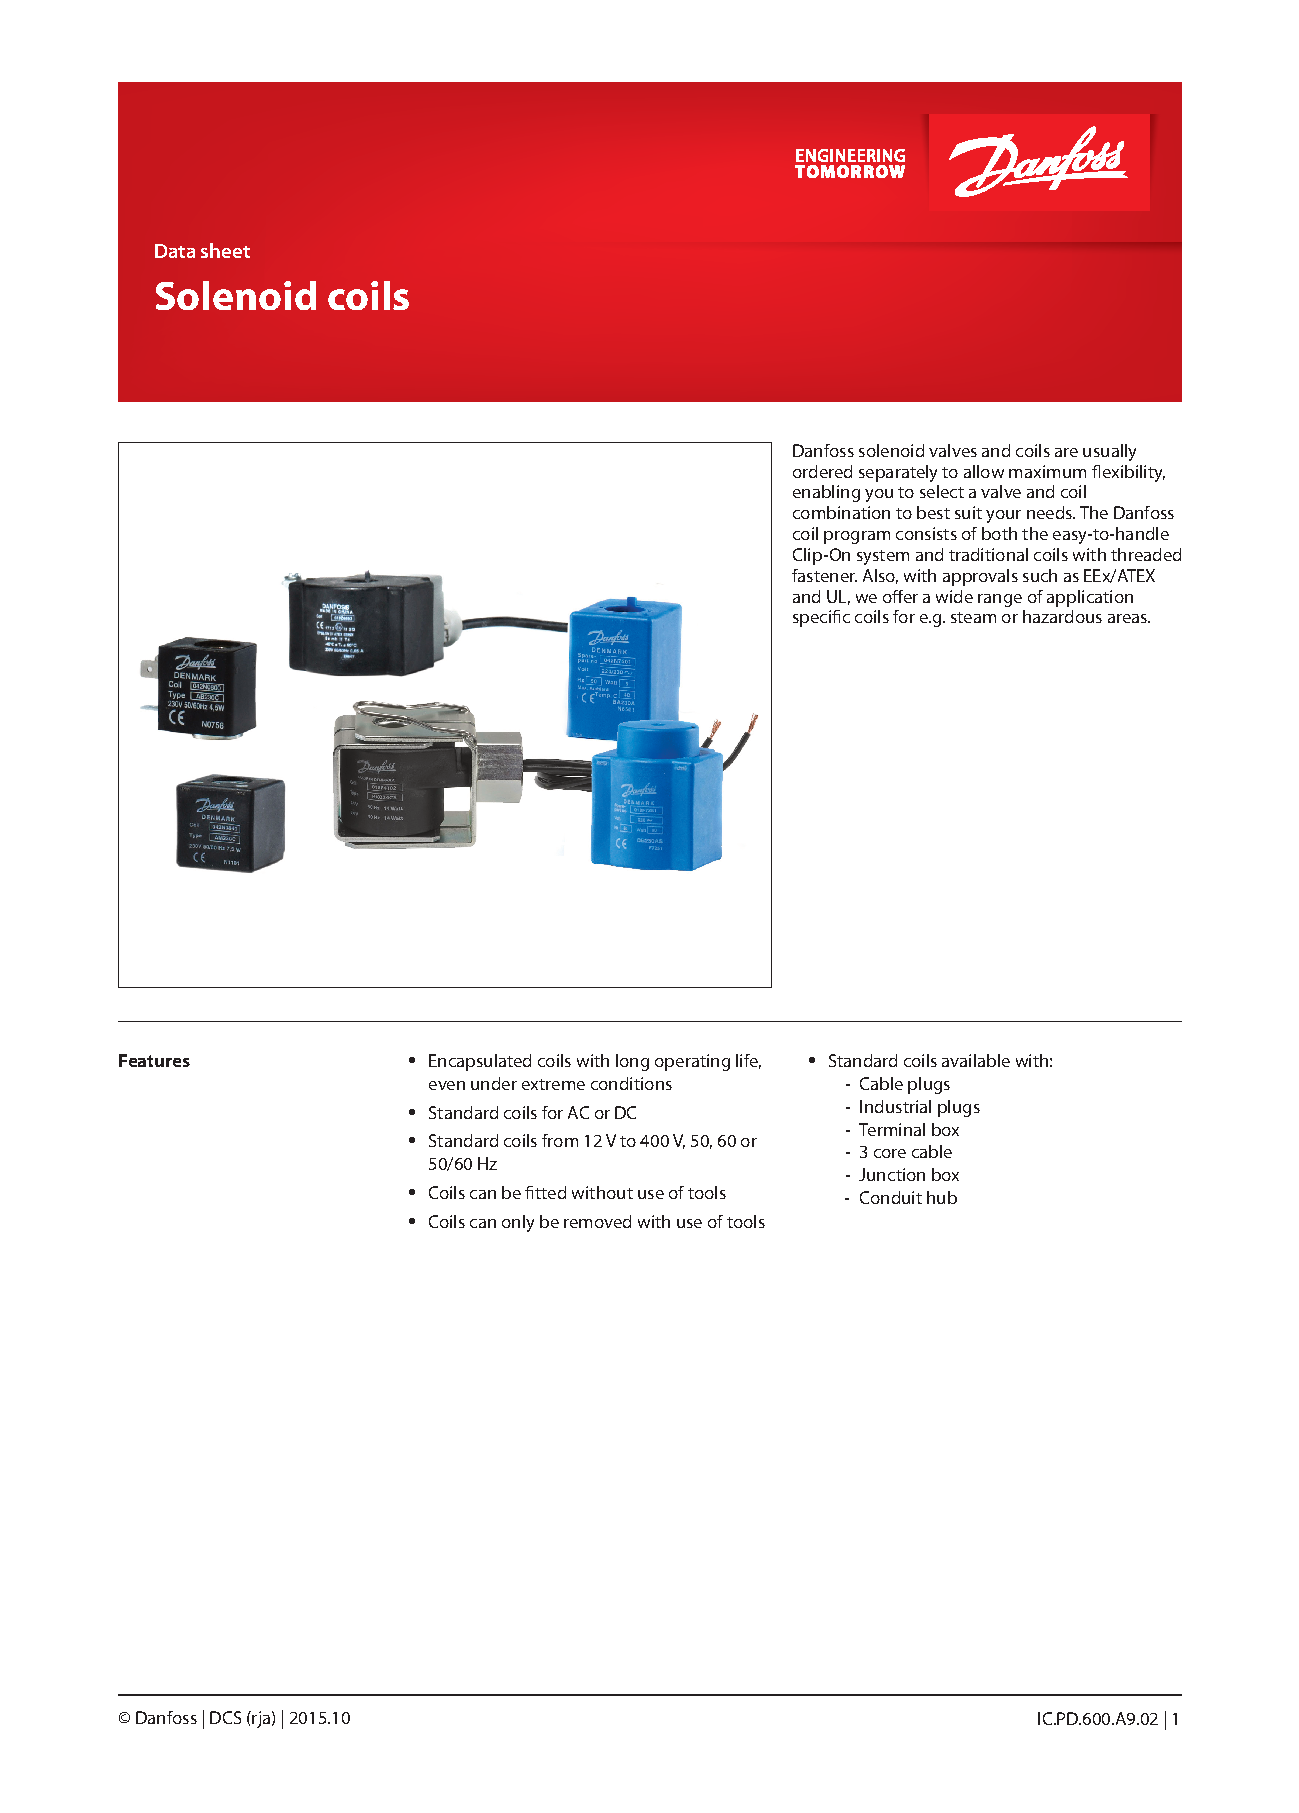
\includepdf[pages=1-2]{./Resources/bobina_danfoss.pdf}

%%%%%%%%%%%%%%%%%%%%%%%%%%%%%%%%%%%%%%%%%%%%%%%%%%%%%%%%%%%%%%%%%%%%%%%%%%%%%

\chapter{Bomba centr\'ifuga Topsflo B08H\-12\-1006}
\label{Anexo5}

%Adiciona o PDF do diagrama esquemático da BBB
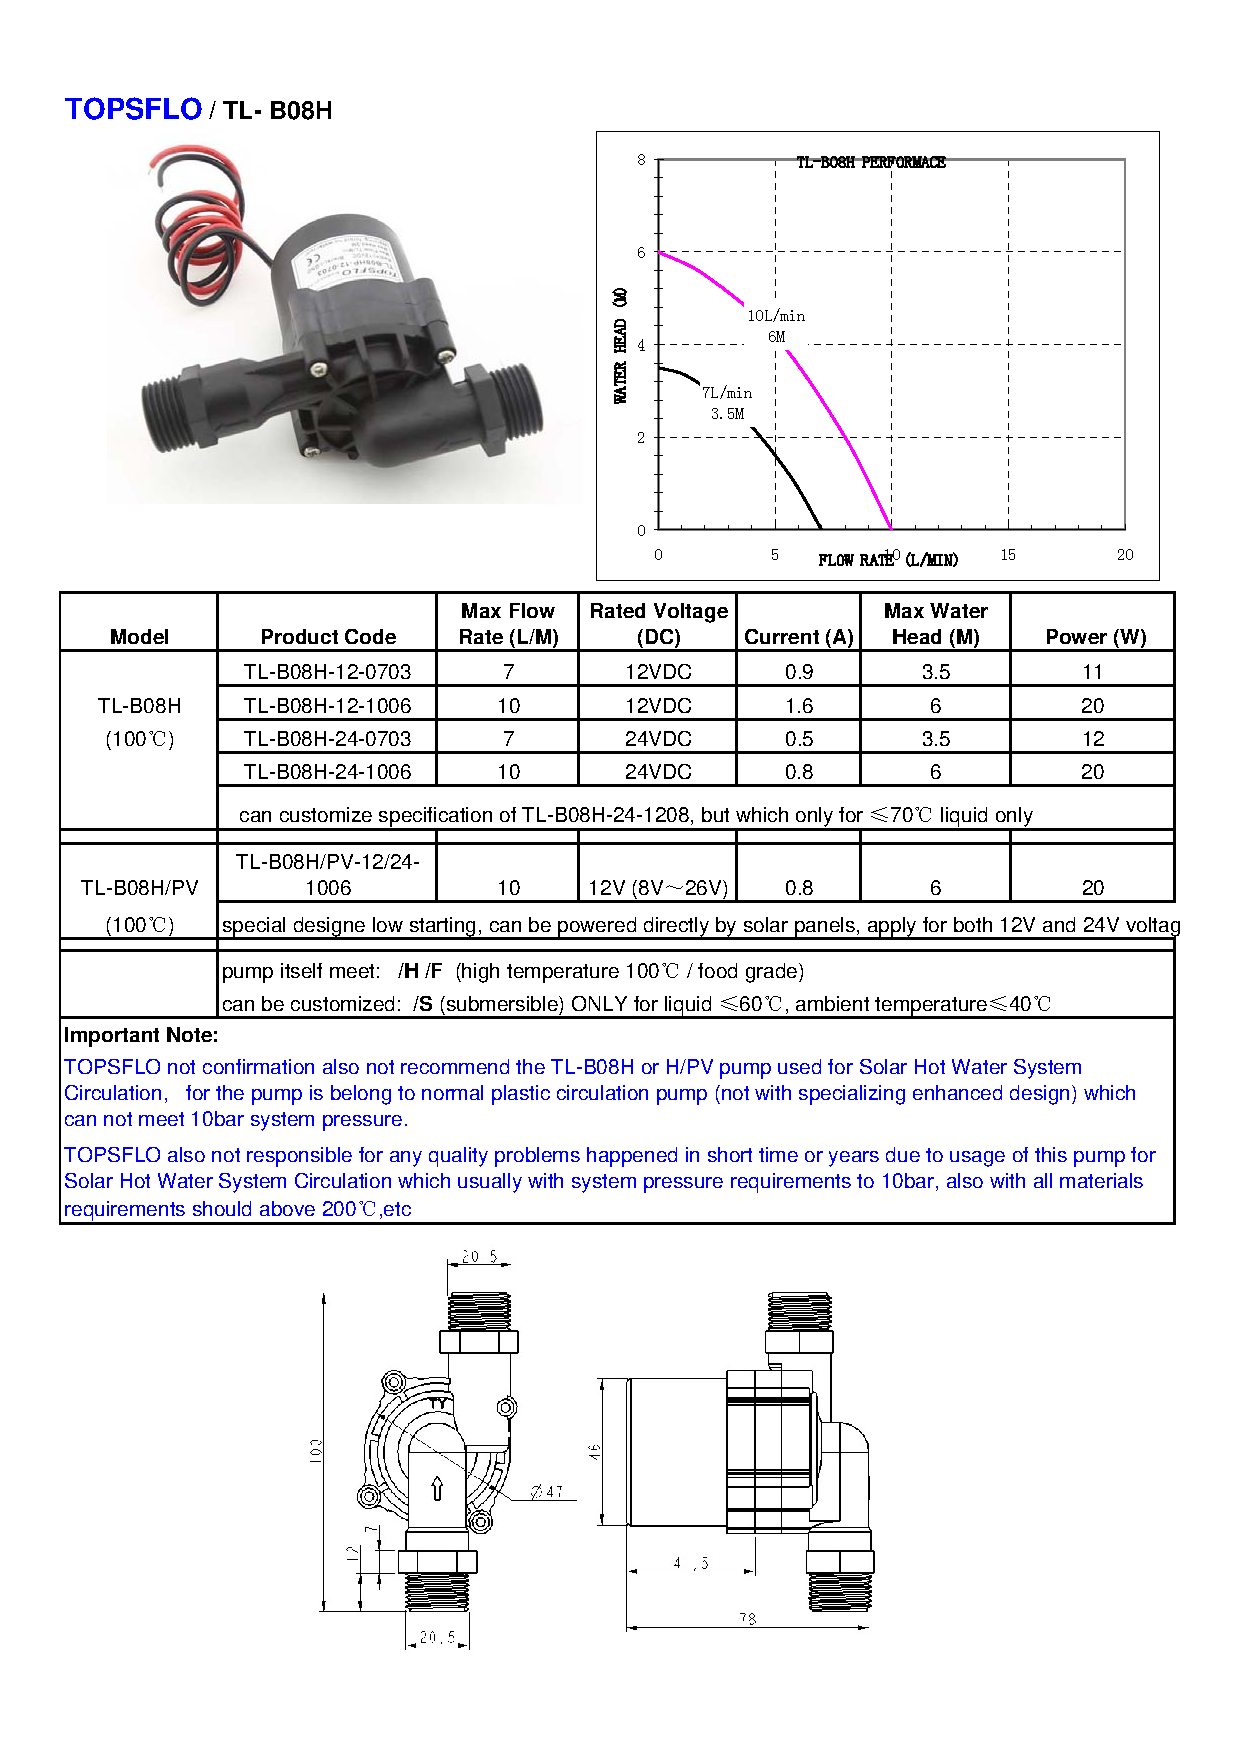
\includepdf[pages=-]{./Resources/TL-B08H.pdf}

%%%%%%%%%%%%%%%%%%%%%%%%%%%%%%%%%%%%%%%%%%%%%%%%%%%%%%%%%%%%%%%%%%%%%%%%%%%%%
